\documentclass[12pt]{article}
\usepackage[utf8]{inputenc}
\usepackage{float}
\usepackage{amsmath}

\usepackage[hmargin=3cm,vmargin=6.0cm]{geometry}
%\topmargin=0cm
\topmargin=-2cm
\addtolength{\textheight}{6.5cm}
\addtolength{\textwidth}{2.0cm}
%\setlength{\leftmargin}{-5cm}
\setlength{\oddsidemargin}{0.0cm}
\setlength{\evensidemargin}{0.0cm}

%misc libraries goes here
\usepackage{fitch}
\usepackage{tikz}

\begin{document}

\section*{Student Information } 
%Write your full name and id number between the colon and newline
%Put one empty space character after colon and before newline
Full Name : Mithat Can Timurcan\\
Id Number :  2581064\\

% Write your answers below the section tags
\section*{Answer 1}
\paragraph*{a)}
\begin{itemize}
    \item \textbf{Base Case ($n = 1$):}
    \begin{equation*}
        \begin{split}
         2^3 - 3 = 5\\
        \end{split}
    \end{equation*}
    \begin{itemize}
        \item Since 5 is divisible by itself, we can see that the base case holds.
    \end{itemize}
    \item \textbf{Inductive Step ($n \geq 1$):}
    \begin{itemize}
        \item Assume that the property holds for some integer $k \geq 1$. We have the following:
        \begin{equation*}
            \begin{split}
            5 \ | \ 2^{3k} - 3^k
            \end{split}
        \end{equation*}
        \item Then we can see that for some integer $c$:
        \begin{equation*}
            \begin{split}
            2^{3k} - 3^k = 5c
            \end{split}
        \end{equation*}
        \item Let's also consider for the integer $k + 1$:
        \begin{equation*}
            \begin{split}
            2^{3(k+1)} - 3^{(k+1)} = 2^3\cdot2^{3k} - 3\cdot3^k 
            \end{split}
        \end{equation*}
        \item We can replace $2^{3k}$ with $3^k + 5c$ (inductive hypothesis):
        \begin{equation*}
            \begin{split}
            8 \cdot (3^k + 5c) - 3 \cdot 3^k = 5 \cdot 3^k + 40c = 5(3^k + 8c)
            \end{split}
        \end{equation*}
        \item We can see that $5(3^k + 8)$ is divisible by 5.
    \end{itemize}
    \item Therefore, we have shown that $2^{3n} - 3^n$ is divisible by 5 for all integers $n \geq 1$ by using mathematical induction.
\end{itemize}
\paragraph*{b)}
\begin{itemize}
    \item \textbf{Base Case ($n = 2$):}
    \begin{equation*}
        \begin{split}
         4^2 - 7 \cdot 2 - 1 = 1 > 0 
        \end{split}
    \end{equation*}
    \begin{itemize}
        \item We can see that the base case holds.
    \end{itemize}
    \item \textbf{Inductive Step ($n \geq 2$):}
    \begin{itemize}
        \item Assume that the property holds for some integer $k \geq 2$. We have the following:
        \begin{equation*}
            \begin{split}
             4^k - 7k - 1 > 0 
            \end{split}
        \end{equation*}
        \item Let's also consider for the integer $k + 1$.
        \begin{equation*}
            \begin{split}
             4^{k+1} - 7(k+1) - 1 = 4 \cdot 4^k - 7k - 8
            \end{split}
        \end{equation*}
        \item We can manipulate the inductive hypothesis as follows:
        \begin{equation*}
            \begin{split}
             4^k > 7k + 1\\
             4 \cdot 4^k > 28k + 4
            \end{split}
        \end{equation*}
        \item Going back to our equation using the inductive hypothesis:
        \begin{equation*}
            \begin{split}
                4 \cdot 4^k - 7k - 8 > 28k + 4 - 7k - 8 = 21k - 4 > 0
            \end{split}
        \end{equation*}
        \item Since $k \geq 2$ for all $k$ values, we can see that $21k-4 > 0$ for all $k$ values and therefore, $4^{k+1} - 7(k+1) - 1 > 0$.
    \end{itemize}
    \item Therefore, we have shown that $4^n - 7n - 1 > 0$ for all integers $n \geq 2$ by using mathematical induction.
\end{itemize}
\section*{Answer 2}
\paragraph*{a)}
\begin{itemize}
 \item In order to find the number of bit strings of length 10 which have at least seven 1s, we can consider the cases where:
 \begin{itemize}
  \item Bit string has 7 1's.
  \item Bit string has 8 1's.
  \item Bit string has 9 1's.
  \item Bit string has 10 1's.
 \end{itemize}
\item Let's calculate each one of the cases:
 \begin{itemize}
  \item We can choose 7 positions for the ones, and the rest of them will be zeros.
  \begin{equation*}
   \begin{split}
   C(10, 7) = \begin{pmatrix} 10 \\ 7 \end{pmatrix} = \dfrac{10!}{(10-7)! \cdot 7!} = 120
   \end{split}
  \end{equation*}
  \item We can choose 8 positions for the ones, and the rest of them will be zeros.
  \begin{equation*}
   \begin{split}
   C(10, 8) = \begin{pmatrix} 10 \\ 8 \end{pmatrix} = \dfrac{10!}{(10-8)! \cdot 8!} = 45
   \end{split}
  \end{equation*}
  \item We can choose 9 positions for the ones, and one position to be zero.
  \begin{equation*}
   \begin{split}
   C(10, 9) = \begin{pmatrix} 10 \\ 9 \end{pmatrix} = \dfrac{10!}{(10-9)! \cdot 9!} = 10
   \end{split}
  \end{equation*}
  \item We can set all of the positions for the ones.
  \begin{equation*}
   \begin{split}
   C(10, 10) = \begin{pmatrix} 10 \\ 10 \end{pmatrix} = 1
   \end{split}
  \end{equation*}
 \end{itemize}
 \item Summing all of the results up, we get $120 + 45 + 10 + 1 = 176$ bit strings.
\end{itemize}
\paragraph*{b)}
\begin{itemize}
 \item Since 2 positions are taken by 1 Discrete Mathematics textbook and 1 Statistical Methods textbook, we have 2 positions left.
 \item We are going to pick 2 textbooks for our collections which can be done by either:
 \begin{itemize}
  \item 1 Discrete Mathematics textbook and 1 Statistical Methods textbook
  \item 2 Discrete Mathematics textbooks
  \item 2 Statistical Methods textbooks
 \end{itemize}
 \item So, there are 3 ways to form our collection of Discrete Mathematics and Statistical Methods textbooks.
\end{itemize}
\paragraph*{c)}
\begin{itemize}
 \item We can calculate the number of onto functions from set from $A \rightarrow B$ where $|A|=m$ and $|B|=n$ by using inclusion-exclusion principle with the following formula:
\begin{equation*}
   \begin{split}
   \sum_{k=0}^{n}{(-1)^k \begin{pmatrix} n \\ k \end{pmatrix} (n-k)^m}
   \end{split}
\end{equation*}
\item Plugging in $m = 5$, $n = 3$ we get:
\begin{equation*}
   \begin{split}
   \begin{pmatrix} 3 \\ 0 \end{pmatrix}3^5 - \begin{pmatrix} 3 \\ 1 \end{pmatrix}(3-1)^5 + \begin{pmatrix} 3 \\ 2 \end{pmatrix}(3-2)^5 - \begin{pmatrix} 3 \\ 3 \end{pmatrix}(3-3)^5 = 243 - 96 + 3 - 0= 150
   \end{split}
\end{equation*}
\item So, there are 150 onto functions that can be defined from a set with 5 elements to a set with 3 elements.
\end{itemize}
\section*{Answer 3}
\begin{center}
    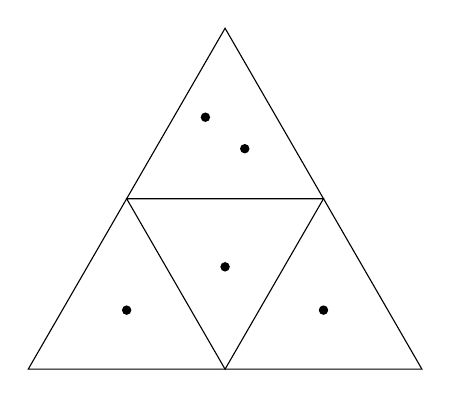
\begin{tikzpicture}
    \draw[fill=white!50]
        (0,0)   -- coordinate (a) ++
        (+60:5) -- coordinate (b) ++
        (-60:5) -- coordinate (c) cycle;
    \draw[black] (a) -- (b) -- (c) -- cycle;
    \coordinate (D1) at (2.25,3.2);
    \coordinate (D2) at (2.75,2.8);
    \coordinate (D3) at (1.25,0.75);
    \coordinate (D4) at (2.5,1.3);
    \coordinate (D5) at (3.75,0.75);
    \foreach \dot in {D1,D2,D3,D4,D5}
        \fill (\dot) circle (0.06);
    \end{tikzpicture}
    \\ \textbf{Figure 1.} An equilateral triangle with side length of 500 meters.
    \end{center}
    \begin{itemize}   
     \item From Figure 1. it can be observed that there are 4 holes (equilateral triangle spots with side length of 250 meters) and 5 pigeons (children). By the Pigeonhole Principle, there must be at least 2 pigeons in the same hole.
     \item When 2 children are at the same hole, their distance can not exceed 250 meters, their max distance will be 250 meters and this occurs when they're at the corners of the hole.
    \end{itemize}
\section*{Answer 4}
\begin{itemize}
    \item Let's consider the recurrence:
    \begin{equation*}
        \begin{split}
            a_n = 3a_{n-1} + 5^{n-1}\\
            a_n - 3a_{n-1} = 5^{n-1}
        \end{split}
    \end{equation*}
\end{itemize}
\paragraph*{a)}
\begin{itemize}
    \item Homogeneous equation: $a_n - 3a_{n-1} = 0$
    \item Characteristic polynomial can be given as $\lambda - 3 = 0$ so the only characteristic root is $\lambda = 3$.
    \item Therefore, the solution is of the form $a_n^{(h)} = c_1\cdot3^n$.
\end{itemize}
\paragraph*{b)}
\begin{itemize}
    \item Since 5 is not a characteristic root, the particular solution will be of the form $a_n^{(p)} = c_2\cdot5^n$.
    \item Plugging into the recurrence relation:
    \begin{equation*}
        \begin{split}
            c_2\cdot5^n - 3(c_2\cdot5^{n-1}) = 5^{n-1}\\
            c_2\cdot5^n - \dfrac{3c_2\cdot5^n}{5} = \dfrac{5^n}{5}\\
            \dfrac{2c_2\cdot5^n}{5} = \dfrac{5^n}{5}\\
            c_2 = \dfrac{1}{2}
        \end{split}
    \end{equation*}
    \item Since we found both homogeneous and particular solutions, we can sum them up and find the total solution.
    \begin{equation*}
        \begin{split}
            a_n = a_n^{(h)} + a_n^{(p)} = c_1\cdot3^n + \dfrac{5^n}{2} \ \text{with the initial condition $a_1 = 4$}\\
            a_1 = 3c_1 + \dfrac{5}{2} = 4 \ \text{we get $c_1 = \dfrac{1}{2}$} \rightarrow
            a_n = \dfrac{3^n}{2} + \dfrac{5^n}{2}
        \end{split}
    \end{equation*}
\end{itemize}
\paragraph*{c)}
\begin{itemize}
    \item \textbf{Base Case ($n = 1$):}
    \begin{equation*}
        \begin{split}
            \dfrac{3^1}{2} + \dfrac{5^1}{2} = 4
        \end{split}
    \end{equation*}
    \begin{itemize}
        \item We can see that the base case satisfies the initial condition $a_1 = 4$.
    \end{itemize}
    \item \textbf{Inductive Step ($n \geq 1$):}
    \begin{itemize}
        \item Assume that the property holds for some integer $k \geq 1$.
        \item Then we have the following:
        \begin{equation*}
            \begin{split}
                a_k = \dfrac{3^k + 5^k}{2}
            \end{split}
        \end{equation*}
        \item Now using inductive hypothesis, let's show that it holds for the integer $k+1$:
        \begin{equation*}
            \begin{split}
                a_{k+1} - 3a_k = 5^k\\
            \end{split}
        \end{equation*}
        \begin{equation*}
            \begin{split}
                a_{k+1} = \dfrac{3(3^k + 5^k)}{2} + 5^k = \dfrac{3^{k+1} + 3\cdot5^k + 2\cdot5^k}{2} = \dfrac{3^{k+1} + 5^{k+1}}{2}
            \end{split}
        \end{equation*}
    \end{itemize}
    \item Therefore, we have shown that $a_n = \dfrac{3^n}{2} + \dfrac{5^n}{2}$ is a solution for all $n \geq 1$.
\end{itemize}
\end{document}
